The technology behind eKwip is able to capture the movements of the knee and allow athletes and their physicians to monitor the motion of the leg. The system consists of several sub-components, each of which performs an important function as part of the system as a whole. The sub-components include a spandex wrap, a microcontroller, sensors, a wireless module, and a webserver.

Figure~\ref{fig:block_diagram} shows a block diagram modelling the eKwip system.

\begin{figure}[h]
  \begin{center}
    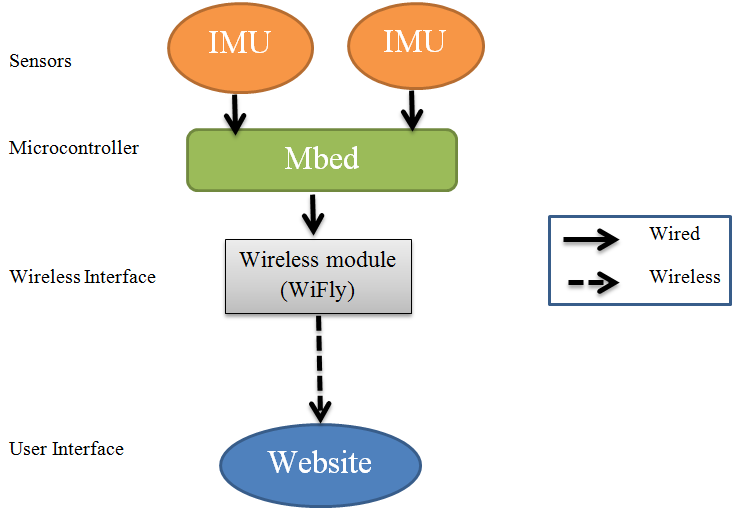
\includegraphics[width=3in]{images/block_diagram.PNG}
  \end{center}
  \caption{Block diagram of eKwip system}
  \label{fig:block_diagram}
\end{figure}

\subsection {Wrap}
In order to measure the movements of the leg and knee, a wrap is required to wrap around the leg and position the sensors appropriately. Since it is required to have a sensor on the upper leg and a sensor on the lower leg, so the relative position and movement can be measured, a wrap allows the correct placement of the sensors and keeps the sensors stationary.

\subsection {Microcontroller}
A microcontroller is required for eKwip so that the data collected is processed and transmitted elsewhere for further analysis. The microcontroller receives input from the sensors while simultaneously sending data out through its serial lines to the wireless module.

\subsection {Sensors}
eKwip requires two sensors in order to successfully model the position and movement of the leg and knee, because the relative motion of the upper and lower leg must be measured. The sensors are required to be able to measure acceleration, absolute orientation, and rate of change of the absolute orientation.

\subsection {Wireless Module}
After collecting the data, it needs to be transmitted elsewhere for further processing and analysis. A wireless module allows the microcontroller to stream data in real time over the internet to the server. Because of this, eKwip is able to display the motion of the leg and all pertinent data to the user in real time.

\subsection {Server}
For data visualization and extraction, a server is used. The server collects the data that is transmitted from the wireless module, processes it, and displays the motion of the leg to the user. Additionally, the server allows for the storage and retrieval of the raw data so it can be analyzed.
